\documentclass{article}
\usepackage{graphicx}
\usepackage{wrapfig}
\usepackage{filecontents}
\usepackage{siunitx}
\usepackage[table]{xcolor}
\usepackage{float}
\usepackage{hyperref}

\usepackage{color} % balíček pro obarvování textů
\usepackage{xcolor}  % zapne možnost používání barev, mj. pro \definecolor
\usepackage{pgfplots} % http://www.chiark.greenend.org.uk/doc/texlive-doc/latex/pgfplots/pgfplots.pdf

\ifnum 0\ifxetex 1\fi\ifluatex 1\fi=0 % if pdftex
  \usepackage[T1]{fontenc}
  \usepackage[utf8]{inputenc}
\else % if luatex or xelatex
  \ifxetex
    \usepackage{mathspec}
  \else
    \usepackage{fontspec}
  \fi
  \defaultfontfeatures{Ligatures=TeX,Scale=MatchLowercase}
\fi
\usepackage[total={175mm,230mm}, top=23mm, left=20mm, includefoot]{geometry}
\hypersetup{
    colorlinks,
    linkcolor={blue!50!black},
    citecolor={green!50!black},
    urlcolor={blue!80!black}
}
% \definecolor{fialova}{RGB}{ 255, 000, 255}
\definecolor{color-si1}{RGB}{ 255, 000, 000}
\definecolor{color-si2}{RGB}{ 251, 130, 032}

\definecolor{color-ge1}{RGB}{ 000, 255, 000}
\definecolor{color-ge2}{RGB}{ 032, 251, 160}

\definecolor{color-inp1}{RGB}{ 000, 000, 255}
\definecolor{color-inp2}{RGB}{ 160, 032, 251}

\definecolor{color-geas1}{RGB}{ 225, 225, 000}
\definecolor{color-geas2}{RGB}{ 225, 225, 100}

\definecolor{sedak}{RGB}{ 100, 100, 100}


\newcommand \obr[1]
{ obr.~\ref{#1}}

\newcommand \tab[1]
{ tab.~ß\ref{#1}}


\begin{document}
\pagestyle{empty}

\definecolor{color_29791}{rgb}{0,0,0}
\begin{figure}[H]
    \hspace{-13mm}
    \begin{minipage}[t]{\textwidth}
        \vspace{-20mm}
        \begin{tikzpicture}[overlay]
            \path(0pt,0pt);
        \end{tikzpicture}
        \begin{picture}(-5,0)(2.5,0)
            \put(123.656,-82.75397){\fontsize{18}{1}\usefont{T1}{ptm}{m}{n}\selectfont\color{color_29791}VYSOKÉ UČENÍ TECHNICKÉ V BRNĚ}
            \put(76.296,-104.785){\fontsize{13}{1}\usefont{T1}{ptm}{m}{n}\selectfont\color{color_29791}FAKULTA  ELEKTROTECHNIKY A KOMUNIKAČNÍCH TECHNOLOGIÍ}
            \put(198.447,-128.5339){\fontsize{16}{1}\usefont{T1}{cmr}{b}{n}\selectfont\color{color_29791}Ústav elektrotechnologie}
            \put(156.848,-278.1589){\fontsize{14}{1}\usefont{T1}{ptm}{m}{n}\selectfont\color{color_29791}LABORATORNÍ CVIČENÍ Z PŘEDMĚTU}
            \put(83.123,-300.2579){\fontsize{14}{1}\usefont{T1}{cmr}{b}{n}\selectfont\color{color_29791}ELEKTROTECHNICKÉ MATERIÁLY A VÝROBNÍ PROCESY}
            \put(55.85,-421.25){\fontsize{14}{1}\usefont{T1}{cmr}{b}{n}\selectfont\color{color_29791}Číslo úlohy: 6}
            \put(55.85,-469.547){\fontsize{14}{1}\usefont{T1}{cmr}{b}{n}\selectfont\color{color_29791}Název úlohy: Počítačové vytváření pásových modelů polovodičových materiálů}
            \put(23.9,-620.32){\fontsize{12}{1}\usefont{T1}{cmr}{b}{n}\selectfont\color{color_29791}Jméno a příjmení, ID:}
            \put(23.9,-637.119){\fontsize{12}{1}\usefont{T1}{cmr}{b}{n}\selectfont\color{color_29791}Tomáš Vavrinec, 240893}
            \put(186.95,-620.32){\fontsize{12}{1}\usefont{T1}{cmr}{b}{n}\selectfont\color{color_29791}Atmosférický tlak:}
            \put(186.95,-637.119){\fontsize{12}{1}\usefont{T1}{cmr}{b}{n}\selectfont\color{color_29791}102.6 hPa}
            \put(293.25,-620.32){\fontsize{12}{1}\usefont{T1}{cmr}{b}{n}\selectfont\color{color_29791}Teplota okolí: }
            \put(293.25,-637.119){\fontsize{12}{1}\usefont{T1}{cmr}{b}{n}\selectfont\color{color_29791}25.1°C}
            \put(417.25,-620.32){\fontsize{12}{1}\usefont{T1}{cmr}{b}{n}\selectfont\color{color_29791}Relativní vlhkost:}
            \put(417.25,-637.119){\fontsize{12}{1}\usefont{T1}{cmr}{b}{n}\selectfont\color{color_29791}37.2\%}
            \put(23.9,-665.77){\fontsize{12}{1}\usefont{T1}{cmr}{b}{n}\selectfont\color{color_29791}Měřeno dne:}
            \put(23.9,-682.569){\fontsize{12}{1}\usefont{T1}{cmr}{b}{n}\selectfont\color{color_29791}14.10.2022}
            \put(186.95,-665.77){\fontsize{12}{1}\usefont{T1}{cmr}{b}{n}\selectfont\color{color_29791}Odevzdáno dne:}
            \put(293.25,-665.77){\fontsize{12}{1}\usefont{T1}{cmr}{b}{n}\selectfont\color{color_29791}Ročník, stud. skupina:}
            \put(293.25,-682.569){\fontsize{12}{1}\usefont{T1}{cmr}{b}{n}\selectfont\color{color_29791}2}
            \put(417.25,-665.77){\fontsize{12}{1}\usefont{T1}{cmr}{b}{n}\selectfont\color{color_29791}Kontrola:}
            \put(23.9,-703.42){\fontsize{12}{1}\usefont{T1}{cmr}{b}{n}\selectfont\color{color_29791}Spolupracovali:}
            \put(23.9,-720.219){\fontsize{12}{1}\usefont{T1}{cmr}{b}{n}\selectfont\color{color_29791}Daniel Poisl}
        \end{picture}
        \begin{tikzpicture}[overlay]
            \path(0pt,0pt);
            \draw[color_29791,line width=0.5pt]
            (20.4pt, -606.117pt) -- (20.4pt, -722.815pt)
            ;
            \draw[color_29791,line width=0.5pt]
            (183.45pt, -606.117pt) -- (183.45pt, -651.067pt)
            ;
            \draw[color_29791,line width=0.5pt]
            (183.45pt, -651.567pt) -- (183.45pt, -688.717pt)
            ;
            \draw[color_29791,line width=0.5pt]
            (289.75pt, -606.117pt) -- (289.75pt, -651.067pt)
            ;
            \draw[color_29791,line width=0.5pt]
            (289.75pt, -651.567pt) -- (289.75pt, -688.717pt)
            ;
            \draw[color_29791,line width=0.5pt]
            (413.75pt, -606.117pt) -- (413.75pt, -651.067pt)
            ;
            \draw[color_29791,line width=0.5pt]
            (413.75pt, -651.567pt) -- (413.75pt, -688.717pt)
            ;
            \draw[color_29791,line width=0.5pt]
            (544.9pt, -606.117pt) -- (544.9pt, -722.815pt)
            ;
            \draw[color_29791,line width=0.5pt]
            (20.15pt, -605.867pt) -- (545.15pt, -605.867pt)
            ;
            \draw[color_29791,line width=0.5pt]
            (20.65pt, -651.317pt) -- (544.65pt, -651.317pt)
            ;
            \draw[color_29791,line width=0.5pt]
            (20.65pt, -688.967pt) -- (544.65pt, -688.967pt)
            ;
            \draw[color_29791,line width=0.5pt]
            (20.15pt, -723.065pt) -- (545.15pt, -723.065pt)
            ;
            \draw[color_29791,line width=1.5pt]
            (15.75pt, -15.59998pt) -- (15.75pt, -729pt)
            ;
            \draw[color_29791,line width=1.5pt]
            (549.55pt, -15.59998pt) -- (549.55pt, -729pt)
            ;
            \draw[color_29791,line width=1.5pt]
            (15.75pt, -729pt) -- (549.55pt, -729pt)
            ;
            \draw[color_29791,line width=1.5pt]
            (15pt, -14.84998pt) -- (550.3pt, -14.84998pt)
            ;
        \end{tikzpicture}
    \end{minipage}
\end{figure}

\newpage
\pagestyle{plain}


\section*{Zadání}
S pomocí grafické metody stanovte pro vybrané izolační materiály bod v jejich H-N diagramu
pro který platí \((\omega \tau) = 1\), a na základě parametrů tohoto bodu odsimulujte pomocí programu
Havriliak-Negami.bat hodnoty distribučních parametrů \(\alpha\) a \(\beta\).
Vyhodnoťte, jak se liší simulovaný průběh od naměřeného a pokuste se na H-N diagramu najít
bod pro který dojde k co nejlepší shodě mezi simulovaným a naměřeným průběhem. Zhodnoťte
jak se od sebe liší graficky odečtený bod \((\omega \tau) = 1\) a bod nejlepší shody.
Na základě hodnot \(\alpha\) a \(\beta\) pro bod nejlepší shody vypočtěte kmitočtovou závislost dielektrické
konstanty \(\epsilon`\) a ztrátového čísla \(\epsilon``\) na kmitočtu (minimálně pro 20 hodnot) a sestrojte H-N
diagram.

\section*{Teoretický úvod}


\newpage
\subsection*{Podmínky měření}
% \begin{tabular}{|c|c|c|}
%     \hline
%     Teplota \(25.1\-[^\circ C]\) & vzdušná vlhkost \(37.2\-[\%RH]\) & atm. tlak \(p = 102.6\-[hPa]\) \\ \hline
% \end{tabular}

\begin{figure}[H]
    % \hfill
    \begin{minipage}[t]{\textwidth}
        \centering
        \begin{tikzpicture}
            \begin{axis}[
                width=\textwidth, 
                height=0.6\textwidth,
                title={chloprenový kaučuk},
                xlabel={\(T\-[K]\)}, 
                ylabel={\(W\-[eV]\)},
                xmin=2.5, xmax=6.2,
                ymin=0.0, ymax=0.7,
                xtick={0,0.2,...,6.5},
                ytick={0,0.1,...,1.5},
                legend pos=north west,
                ]
                \addplot[
                color=blue,
                ]
                coordinates {
                    (6.10, 0.00)
                    (5.85, 0.26)
                    (5.66, 0.42)
                    (5.51, 0.50)
                    (5.33, 0.57)
                    (5.24, 0.59)
                    (5.10, 0.63)
                    (4.94, 0.65)
                    (4.75, 0.66)
                    (4.52, 0.65)
                    (4.22, 0.61)
                    (3.85, 0.53)
                    (3.65, 0.46)
                    (3.46, 0.40)
                    (3.36, 0.36)
                    (3.12, 0.27)
                    (2.91, 0.20)
                    (2.80, 0.15)
                    (2.63, 0.08)
                    (2.53, 0.04)
                };
            \addplot[
                    dotted,
                    thick,
                    color=black,
                ]
                coordinates {
                    (2.43 , 0)
                    (2.53 , 0.04)
                    (4.8  , 1)
                };
            \addplot[
                dotted,
                thick,
                color=black,
                ]
                coordinates {
                    (2.4  , 0)
                    (7    , 0.75)
                };
            \addplot[
                    dotted,
                    thick,
                    color=black,
                    mark=o
                ]
                coordinates {
                    (5.496, 0)
                    (5.496, 0.505)
                };
            \end{axis}
        \end{tikzpicture}
    \end{minipage}

    \begin{minipage}[t]{\textwidth}
        \centering
        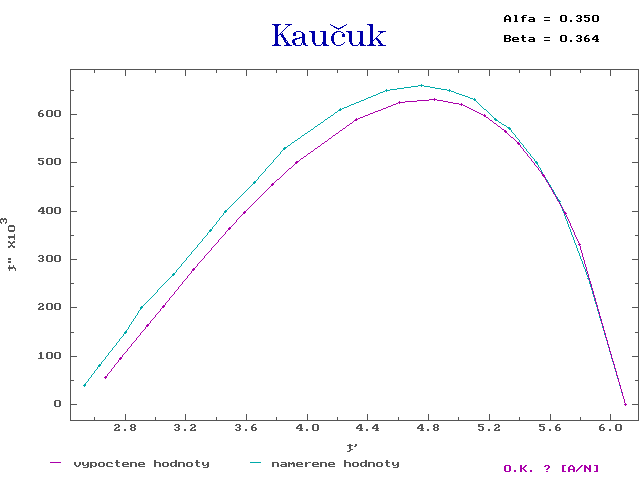
\includegraphics[width=0.8\textwidth]{obrazky/kaucuk_vypoctene.png}
    \end{minipage}
\end{figure}


\subsection*{Závěr}


\end{document}